\providecommand{\main}{../main}
\documentclass[\main/main.tex]{subfiles}
\graphicspath{{../images/}}
\begin{document}
\title{}
\subtitle{Fradkin 14章}
\author{政岡凜太郎}
\frame{\titlepage}
\begin{frame}{目次}\tableofcontents\end{frame}
\subsection*{Constants}
\begin{frame}{\currentname}
    このノートでは自然単位系を用いる。すなわち$ħ = c = ϵ₀ = 1$とする。
    またゲージ場$A_μ$に電荷$e$を含める定義を採用する。
    このとき、$A_μ$は長さの逆数の次元をもつ。形式的には$e$を$1$に置き換えればよい。
    同様に磁場や磁束も全て$e$倍したものを定義として用いる。
    このとき量子Hall系に対する磁気長は$l_B = √{1/B}$となり、磁束量子は$ϕ₀ = 2π$となる。
\end{frame}
\section{14.1 Quantum Hall fluids on a torus}
\begin{frame}{\currentname}
    トーラス$𝕋²(L)$上で定義された$N$粒子の量子Hall系に対して、重心運動の自由度を分離することを考えてみよう。
    各粒子の位置$𝒙_i$に対して、重心の位置$𝑿$は
    \begin{align}
        𝑿 = ÷1{N}∑_{i=1}^N 𝒙_i + ÷{L}{N}𝒏,␣ 𝒏 ∈ (ℤ_N)²
    \end{align}
    と表される。トーラス上では$N$で割る操作は$(ℤ_N)²$の不定性を生むことに注意。
    不定性をなくすために、$𝑿 ∈ [0,L/N)²$を仮定する。
    ここで連続的に$𝒙₁$を$L𝒆_μ$だけ動かすと、もとの配位に戻って来るが、$𝑿$は
    \begin{align}
        𝑿 → 𝑿 + ÷{L}{N}𝒆_μ
    \end{align}
    となる。したがって$𝑿 ∈ 𝕋²(L/N)$とするべきである。

    しかし、このように定義した重心座標$𝑿$と相対座標$𝒙'_i ≔ 𝒙_i - 𝑿$によって$N$粒子の配位を直積$(𝑿,\{𝒙'_i\})$のように表すことはできない。
    これは$\{𝒙'_i\}$を固定したまま、$𝑿$を連続的に$(L/N)𝒆_μ$だけ並進すると分かる。
    このとき$(𝑿,\{𝒙'_i\})$は不変になるはずだが、もとの座標系では
    \begin{align}
        𝒙_i → 𝒙_i - ÷{L}{N}𝒆_μ
    \end{align}
    となる。したがって$(𝑿,\{𝒙'_i\})$は直積ではなく、$L/N$単位の並進によってひねられて貼り合わされている。
    つまり$(𝑿,\{𝒙'_i\})$は$𝕋²(L/N)$を底空間、$(ℤ_N)²$を構造群とするファイバーバンドルになっている。
\end{frame}
\begin{frame}{\currentname}
    次に量子系を考えよう。
    状態空間の基底は$|𝑿⟩|\{𝒙_i-𝑿\}⟩$と書ける。
    ただしこれはテンソル積ではなく、
    \begin{align}
        T(÷{L}{N}𝒆_μ)|𝑿⟩|\{𝒙_i-𝑿\}⟩ = |𝑿⟩T(-÷{L}{N}𝒆_μ)|\{𝒙_i-𝑿\}⟩
    \end{align}
    を満たす。ここで$T$は並進演算子である。
    $|𝑿⟩$を独立に扱うためには、相対運動の状態が$T(-(L/N)𝒆_μ)$の固有状態であると仮定すればよい。$|ψ_𝒌⟩$を$T(-(L/N)𝒆_μ)$に対して固有値$ \exp(2π¡k_μ/N)$をもつ固有状態とすると、
    \begin{align}
        T(÷{L}{N}𝒆_μ)|𝑿⟩|ψ_𝒌⟩ = |𝑿⟩ℯ^{2π¡k_μ/N}|ψ_𝒌⟩
    \end{align}
    となる。よってこの場合$|𝑿⟩$はひねり境界条件に従うとすればよい。
\end{frame}
\begin{frame}{\currentname}
    重心の運動量を表す演算子は$𝑷 ≔ ∑_{i=1}^N 𝒑_i$で与えられる。
    また$𝒑'_i ≔ 𝒑_i - 𝑷/N$とおく。Landauゲージまたは対称ゲージのもとで$𝑨(𝒙)$が$𝒙$に対して線形であることに注意すると、
    \begin{align}
        H &= ÷1{2M}∑_i(𝒑_i-𝑨(𝒙_i))² + V(𝒙'₁,…,𝒙'_N) \∅
        &
        = ÷1{2M}∑_i (÷{𝑷}{N}-𝑨(𝑿)+𝒑'_i-𝑨(𝒙'_i))² + V(𝒙'₁,…,𝒙'_N)\∅
        &
        =  ÷1{2NM}(𝑷-N𝑨(𝑿))² + H'(𝒙'₁,…,𝒙'_N,𝒑'₁,…,𝒑'_N)
    \end{align}
    と書ける。
    ここで、相対運動を表すハミルトニアン$H'$は唯一の基底状態をもつとする。
    このとき基底状態の縮退度は重心運動のみによって決まる。
    占有率が$ν = 1/m$のとき、Landau準位の縮退度は$Φ/ϕ₀ = mN$で与えられる。
    重心の電荷は$N$なので、磁束量子は$ϕ₀/N$で与えられる。
    また基底状態が$(L/N)𝒆_μ$の並進に対して固有値$1$をもつとすれば、重心$(L/N)²$のトーラス上を動くので、全磁束は$Φ/N²$で与えられる。
    よって重心にとってのLandau準位の縮退度は$Φ/(Nϕ₀) = m$である。
    ここから$ν=1/m$のときの縮退度は$m$となる。
\end{frame}
\begin{frame}{\currentname}
    \begin{itemize}
        \item  トーラス上のLaughlin波動関数は$θ$関数で表され、縮退度に対応して$m$個の線形独立な波動関数が構成できるらしい。

        \item non-Abelianの場合は重心系の情報だけから縮退度を求めるのは無理らしい。
    \end{itemize}
\end{frame}
\subsection*{14.1.1 Flux attachment on a torus}
\begin{frame}{\currentname}
    相互作用するフェルミオン系、またはボソン系を考える。
    ただし、ボソンの場合はハードコアの相互作用を仮定する。
    linking-numberは電流$j_μ$に対して
    \begin{align}
        ν_𝐿[j] = ÷1{2π} ∫ \𝑑^3x j_μ(x)b^μ(x) ∈ ℤ
    \end{align}
    で与えられる。
    ここで、$b^μ$は$ϵ_{μνλ}∂^νb^λ = 2πj_μ$によって与えられる。
    粒子の世界線が交わらないとき、$ν_𝐿[j]$はトポロジカル不変量であるから、
    作用を$S[j] ↦ S[j] - 2πsν_𝐿[j]$としても等価な理論が得られるはずである。
    ここで$s$は任意の整数である。
    このとき、粒子の遷移振幅は
    \begin{align}
        W = ∑_{[j]}ℯ^{¡S[j]-2π¡sν_𝐿[j] + ¡ϕ[j]}
    \end{align}
    と表される。ただし$ϕ[j]$は粒子の統計性からくる位相因子である。
    経路積分に以下を挿入することで、補助場$a,b$を導入する。
    \begin{align}
        1 &= ∫ \𝒟{b}∏_μ δ[ϵ_{μνλ}∂^νb^λ - 2πj_μ] \∅
        &
        = 𝒩∫\𝒟{b}\𝒟{a} \exp(÷{¡}{2π}∫\𝑑^3x a^μ[ϵ_{μνλ}∂^νb^λ - 2πj_μ])
    \end{align}
    ただし$\𝒟{b}$はゲージ変換の自由度を除いたものとする。
\end{frame}
\begin{frame}{\currentname}
    すると以下のラグランジアンを得る。
    \begin{align}
        ℒ_{eff}[a,b,j]
        = ÷1{2π}a ∧ 𝑑b - a∧★j - ÷{2s}{4π}b∧𝑑b
    \end{align}
    境界の寄与を無視すると$a ∧ 𝑑b = b ∧ 𝑑a$としてよい。
    $b$についての平方完成
    \begin{align}
       ÷1{4π}(a ∧ 𝑑b + b ∧ 𝑑a - 2s b ∧ 𝑑b)
       &
       = -÷{2s}{4π}(b-÷{a}{2s})∧𝑑(b-÷{a}{2s})
       + ÷{1}{4π×2s}a ∧ 𝑑a
    \end{align}
    から、$b$についてintegrate outすることで
    \begin{align}
        S_{eff}[a] = ÷θ{2}∫ a ∧ 𝑑a ,␣
        θ = ÷1{2π×2s}
    \end{align}
    が得られる。まとめると、
    \begin{align}
        W = ∑_{[j]} ∫\𝒟{a} \exp(¡S[j] + ¡ϕ[j] + ¡S_{eff}[a] - ¡∫a ∧ ★j).
        \label{flux attachment}
    \end{align}
    となる。
    ここでゲージ場$a$に対するChern-Simons項はゲージ不変ではないことに注意。
    (\ref{flux attachment})はflux attachmentの具体的な表示になっている。
    ただし、結局$S[j]$が難しいため厳密性を保ったままこれ以上先には行けないと思われる。
\end{frame}
\begin{frame}{\currentname}
    次にabelianな多成分のChern-Simons理論として最も一般的なものを考え、その性質を考える。
    物理的なゲージ場$A_μ$と統計的なゲージ場$a^I_μ,~ I = 1,…,n$に対し、
    整数の成分をもつ行列$K_{IJ}$とベクトル$t_I$によって指定される以下のラグランジアンを考える。
    \begin{align}
        ℒ_{eff} = - ÷1{4π} K_{IJ}ϵ^{μνλ}a^I_μ∂_νa^J_λ - ÷{1}{2π}t_I ϵ^{μνλ}a^I_μ∂_νA_λ
    \end{align}
    行列$K$のことをそのままだが$K$行列と呼ぶ。また$t_I$のことを電荷ベクトルと呼ぶ。
    まず占有率$ν$を求める。古典的な運動方程式の期待値がゼロになることから、
    \begin{align}
        \⟨÷{δS_{eff}}{δa^I_μ}\⟩
        = - ÷{1}{2π} ⟨K_{IJ}ϵ^{μνλ}∂_ν a^J_λ⟩ - ÷1{2π}t_I ϵ^{μνλ}∂_ν A_λ = 0
    \end{align}
    である。各辺に$t^𝑇 K^{-1}$を左から掛けると、
    \begin{align}
        ÷{t^𝑇 K^{-1} t}{2π} ϵ^{μνλ}∂_ν A_λ  = -÷1{2π} ⟨t_Iϵ^{μνλ}∂_ν a^I_λ⟩ = ÷{δS_{eff}}{δA_μ} = ⟨J_μ⟩.
    \end{align}
    よってHallコンダクタンスと占有率$ν$は
    \begin{align}
        σ_{xy} = ÷{t^𝑇 K^{-1}t}{2π},␣
        ν = t^𝑇 K^{-1}t
    \end{align}
    である。ただし、$ν = 2π⟨J₀⟩/B$を用いた。
\end{frame}
\begin{frame}{\currentname}
    次に、ゲージ場$a^I$と整数の電荷$l_I$によって結合する準粒子励起の自由度を系に追加する。
    $l_I$を準粒子ベクトルと呼ぶ。
    このときラグランジアンは
    \begin{align}
        ℒ_{eff} = - ÷1{4π} K_{IJ}ϵ^{μνλ}a^I_μ∂_νa^J_λ - ÷{1}{2π}t_I ϵ^{μνλ}a^I_μ∂_νA_λ - l_I j^μa^I_μ
    \end{align}
    となる。運動方程式は、
    \begin{align}
        \⟨÷{δS_{eff}[A,a^I]}{δa_μ^I}\⟩
        =  - ÷{1}{2π} ⟨K_{IJ}ϵ^{μνλ}∂_ν a^J_λ⟩ - ÷1{2π}t_I ϵ^{μνλ}∂_ν A_λ - l_I⟨j^μ⟩ = 0.
    \end{align}
    各辺に$t^𝑇 K^{-1}$を左から掛けると、
    \begin{align}
        ⟨J_μ⟩ = ÷{t^𝑇K^{-1}t}{2π}ϵ^{μνλ}∂_ν A_λ + t^𝑇K^{-1}l j^μ.
    \end{align}
    第1項は外場による応答を表している。第2項は準粒子励起の寄与であり、電荷$Q$が
    \begin{align}
        Q = t^𝑇K^{-1}l
    \end{align}
    であることが読み取れる。
\end{frame}
\begin{frame}{\currentname}
    次に準粒子の統計位相を見る。そのためにはWilsonループ
    \begin{align}
        W(Γ,l) = \exp(¡∮_{Γ}l_Ia^I) = \exp(¡∫l_Ia^I ∧ δ(Γ))
    \end{align}
    が絡み合った時の期待値を調べれば良い。
    ここでは古典的な計算を用いる。後で量子的な計算も扱う。
    Wilsonループは$a^I$と電荷$l^I$によって結合するデルタ関数的な電流とみなせる。
    一本のWilsonループを作用に加えた状況を古典的に扱うと、統計的ゲージ場$a^I$が従う運動方程式は以下のようになる。
    \begin{align}
        𝑑a^I = 2π(K^{-1}l)^I δ(Γ)
    \end{align}
    このゲージ場のもとでのもう一本のWilsonループの値は
    \begin{align}
       ∮_{∂Σ} l_I a^I  = ∫_{Σ} l_I 𝑑a^I
       = 2πl^𝑇K^{-1}l ∫_{Σ} δ(Γ)
       = 2πl^𝑇K^{-1}l ⋅     \Link(∂Σ,Γ)
    \end{align}
    となる。粒子の交換に対する位相はこの半分なので、
    \begin{align}
        δ = πl^𝑇K^{-1}l
    \end{align}
    となる。結果は量子論的な計算でも同様である。
\end{frame}

\subsection*{14.1.2 Chern-Simons on a torus}
\begin{frame}{\currentname}
    Chern-Simons理論はトポロジカル場の量子論であり、基底状態の縮退度は空間のトポロジーによって変化する。
    我々が考えたいのは基底状態なので、時間方向は$ℝ$とする。
    また空間を表す多様体を$ℳ_g$とし、その種数を$g$とする。
    まず、$a₀^I$をLagrange未定乗数とみなすことで、
    \begin{align}
        Z(ℳ_g)
        &
        = ∫ \𝒟{a_μ} \exp(÷{¡}{4π}∫_{ℝ × ℳ_g} \𝑑^3x K_{IJ}ϵ^{μνλ}a^I_μ∂_νa^J_λ) \∅
        &
        = ∫  \𝒟{a_i}∏_I δ[ϵ_{ij}∂_ia^I_j]
        \exp(÷{¡}{4π}∫ \𝑑{x₀} ∫_{ℳ_g} \𝑑^2 x K_{IJ}ϵ^{ij}a^I_i ∂₀ a^J_j)
    \end{align}
    となる。\footnote{教科書に従ってここでは$K$行列の符号が逆にしている。符号は結論には影響しない。}
    ただし、この分配関数はゲージ変換$a^I_i ↦ a^I_i + ∂_iΛ$の自由度が入っているため、無限大の定数が掛かっている。
    これを取り除くためには、$𝑑a^I = 0$を満たすゲージ場の配位の中で、$a^I ↦ a^I + 𝑑Λ$を同一視したときの同値類 $=$ de Rahmコホモロジー類の自由度を調べればよい。
    $ℳ$に関するde Rahmコホモロジーを見ると、これは$ H¹(ℳ_g) = ℝ^{2g}$で与えられる。
\end{frame}
\begin{frame}{\currentname}
    de Rahmコホモロジー類の代表元を$b_α$として、
    \begin{align}
        a^I_i = ∑_{α=1}^{2g} \_a^I_α b_{α,i}
    \end{align}
    と表すことができる。
    すると分配関数は、
    \begin{align}
        Z(ℳ) = ∫ ∏_α\𝒟{\_a_α} \exp(÷{¡K_{IJ}}{4π}Ω_{αβ}∫\𝑑{x₀} \_a^I_α∂₀\_a^J_β),␣
        Ω_{αβ} ≔ ∫\𝑑^2 x b_α ∧ b_β
    \end{align}
    と表される。
    ここで、代表元$b_α$としてデルタ関数形式$δ(Γ_α)$を用いることにする。
    $Γ_α$は$ℳ$上の可縮でない閉曲線である。
    すると$Ω_{αβ}$は曲線の交点数で与えられるので、
    \begin{align}
        Ω
        =\( 
           ¡σ_y &   &  \\
             & ⋱ &  \\
             &   & ¡σ_y
        \),␣ ¡σ_y = \( 0&1\\-1&0\)
    \end{align}
    とできる。このとき閉曲線の組ごとに作用への寄与が独立になるため、
    \begin{align}
        Z(ℳ) = Z(𝕋²)^{g},␣ Z(𝕋²) = ∫ \𝒟{\_a₁}\𝒟{\_a₂}\exp(÷{¡K_{IJ}}{4π}∫\𝑑{x₀} (\_a₁^I∂₀\_a₂^J-\_a₂^J∂₀\_a₁^I))
    \end{align}
    となる。よって以降はトーラスについて考える。
\end{frame}
\begin{frame}{\currentname}
    \begin{figure}[H]
        \centering
        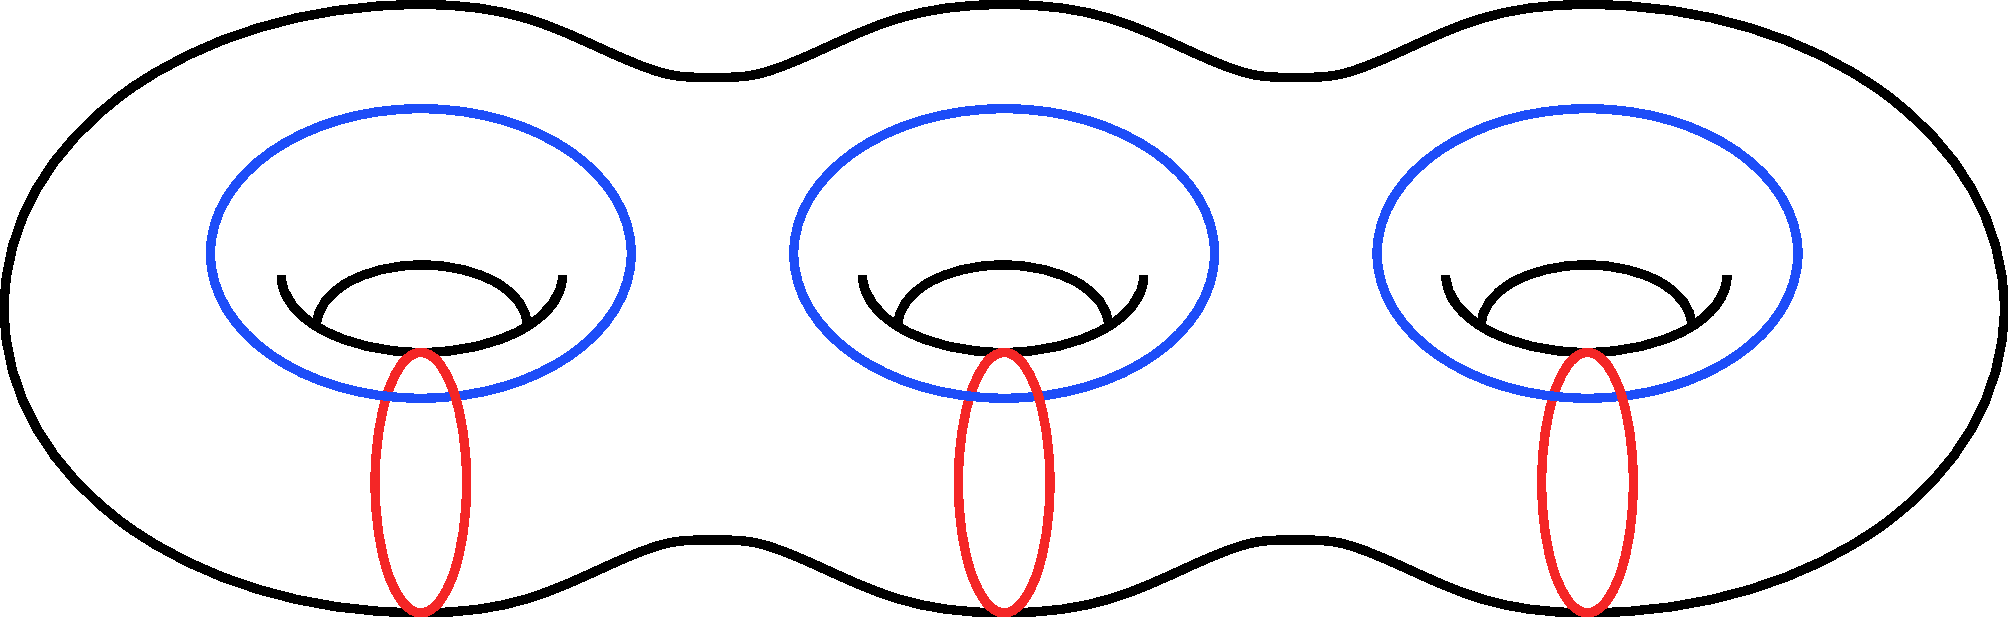
\includegraphics[width=0.7\hsize]{loops.pdf}
    \end{figure}
\end{frame}
\begin{frame}{\currentname}
    変数$\_a₀, \_a₁$の間の正準交換関係は
    \begin{align}
        [\_a_i^I,\_a_j^J] = 2π¡ϵ_{ij}(K^{-1})^{IJ}
    \end{align}
    で与えられる。
    よって
    \begin{align}
        \_a_i^I = 2π¡ϵ_{ij}(K^{-1})^{IJ}÷{∂}{∂\_a_j^J}
    \end{align}
    である。
    ラージゲージ変換$\_a_i^I ↦ \_a_i^I + 2π$に対する不変性から、共役な2つの変数がどちらもコンパクトであることに注意する。
    ここでWilsonループを
    \begin{align}
        W_i^I ≔ ℯ^{¡\_a_i^I} = \exp (¡ ∮_{Γ_i} a)
    \end{align}
    によって定義する。ただし$Γ_i$は$\_a_i^I$が乗っている閉曲線に共役な閉曲線である。
    次に$\_a^I_i ↦ \_a^I_i + 2π$というラージゲージ変換を引き起こす演算子として、
    \begin{align}
        U_i^I ≔ ℯ^{¡ϵ^{ij}(K\_a_j)^I} = ℯ^{2π∂/∂\_a_i}
    \end{align}
    を定義する。
\end{frame}
\begin{frame}{\currentname}
    演算子$U_i^I,~ W_i^I$は以下の関係式を満たす。
    \begin{align}&
        W₁^IW₂^J = ℯ^{-[\_a₁^I,\_a₂^J]}W₂^JW₁^I =  ℯ^{-2π¡K^{-1}_{IJ}}W₂^JW₁^I, \\
        &
        U₁^IU₂^J = ℯ^{[(K\_a₂)^I,(K\_a₁)^J]} U₂^JU₁^I = ℯ^{-2π¡K_{IJ}}U₂^JU₁^I = U₂^JU₁^I, \\
        &
        U_i^IW_j^J = ℯ^{[¡ϵ^{ik}(K\_a_k)^I, ¡\_a_j^I]}W_j^J U_i^I
        = ℯ^{-2π¡δ_{ij}}W_j^JU_i^I = W_j^JU_i^I
    \end{align}
    求めたいのはHilbert空間の次元であった。
    状態は$\_a₁^I$に対する波動関数として表せる。
    $2π$の周期性から、運動量は離散的な整数値$k_I ∈ ℤ$を取る。さらに
    \begin{align}
        \_a₂^I = -2π¡(K^{-1})^{IJ}÷{∂}{∂\_a₁} = 2π(K^{-1})^{IJ}k_J
    \end{align}
    が$2π$の周期性をもつことから、$k_I$は
    \begin{align}
        k_I → k_I + K_{IJ}
    \end{align}
    について周期性をもつ。
    つまり、運動量は$K$の行ベクトルを格子ベクトルとするような周期性をもつ。
    単位格子の中にいる運動量の数は$|\det K|$で与えられるから、Hilbert空間の次元は$|\det K|$である。
    一般の曲面に対するHilbert空間はトーラスのHilbert空間のテンソル積で表されるので、次元は$|\det K|^g$となる。
\end{frame}

\section{14.2 Hydrodynamic theory}
\begin{frame}{\currentname}
    この節では有効理論の視点からChern--Simons理論の妥当性を見ていく。
    まず時空を$S¹ × ℳ$とする。また物理的自由度として電流$J_μ$を採用する。$J_μ$は
    \begin{align}
        J₀(𝒙) = ∑_{i=1}^N δ(𝒙-𝒙_i),␣
        𝑱(𝒙) = ∑_{i=1}^N 𝒗_iδ(𝒙-𝒙_i)
        \label{concrete descrioption of current}
    \end{align}
    と書かれる。また保存則$∂_μJ^μ = 0$が成り立つ。
    系の作用は$S[J]$と表され、電荷の任意の軌道について和をとることで分配関数が得られる。
    ここで保存則$∂_μJ^μ = 0$を満たす場は
    \begin{align}
        J_μ = ÷1{2π}ϵ_{μνλ}∂^νb^λ + ω_μ
    \end{align}
    と表せる。$ω$は調和形式であり、$𝑑ω = 0,~ 𝛿ω = 0$を満たす。
    $J_μ$の具体的表式(\ref{concrete descrioption of current})から$ω$は
    \begin{align}
        ω₀ = ÷{N}{|S¹||ℳ|},␣ 𝝎 = 𝟎
    \end{align}
    に限る。
    また$b$にゲージ変換$b ↦ b + 𝑑Φ$およびラージゲージ変換$b ↦ b + Ω$を行っても$J$は不変である。
    ただし$Ω$は調和形式。よって$S[J]$に対応する$S[b]$はゲージ理論になっている。
\end{frame}

\begin{frame}{\currentname}
    ゲージ理論のラグランジアンで最も素朴なのはMaxwell項$ 𝑑b ∧ ★𝑑b$である。
    $J_μ$は曲面上で積分すると電荷(無次元量)を返すので、自然単位系における次元は$2$である。
    よってゲージ場$b$の次元は$1$である。するとMaxwell項の次元は$4$である。
    しかし、時間反転対称なMaxwell項は磁場中の電子系の有効理論にはなり得ない。
    以下の条件を満たすような作用を考えるとChern--Simons作用のみであることが分かる。
    \begin{itemize}
        \item 時間反転対称性を破る 
        \item パリティを破る
        \item 空間での回転対称性
        \item ゲージ不変性
        \item Maxwell項よりrelevant
    \end{itemize}
    さらに準粒子励起を考えるとどのような有効理論になるだろうか。
    準粒子励起のカレントを$j_μ$とする。
    $j_μ$が統計的ゲージ場$b_μ$のゲージ不変性に付随するカレントであるとき、相互作用項は$qj^μb_μ$と表される。ただし$q$は整数である。よって有効理論のラグランジアンは
    \begin{align}
        ℒ[b_μ,j_μ] = -÷{m}{4π}ϵ^{μνλ}b_μ∂_νb_λ - ÷{1}{2π}ϵ^{μνλ}A_μ∂_νb_λ + qj^μb_μ
    \end{align}
    となる。
\end{frame}

\section{14.3 Hierarchical state}
\begin{frame}{\currentname}
    Laughlin波動関数は占有率が$ν = 1/m$の場合しか記述できない。
    $ν$が$1/m$から微小にずれた場合の波動関数は、希薄な準粒子励起によって記述されていると考えられる。
    Haldaneは$ν$をさらに動かして準粒子励起の密度を大きくしていくと、準粒子励起がLaughling波動関数に従って凝縮すると考えた。
    さらにその状態からの準粒子励起を考え、それが凝縮した状態を考え、というようにいくらでも続けることができる。
    このような状態を階層状態と呼ぶ。
    この描像では$ν$は連分数で表され、顕著なプラトー$ν = 2/5, 3/7, …$をある程度説明できる。
    
    ここでは、Chern--Simons理論と$K$行列の形式によって階層状態を議論する。
    作用は以下のように表される。
    \begin{align}
        ℒ[b_μ, A_μ, j_μ]
        = -÷{m}{4π}ϵ^{μνλ}b_μ∂_νb_λ  - ÷{1}{2π}ϵ_{μνλ}A^μ∂^νb^λ
        + qb_μj^μ + ℒ_{qp-KE}
    \end{align}
    ここで$j^μ$に対して
    \begin{align}
        j_μ = ÷1{2π}ϵ_{μνλ}∂^νc^λ
    \end{align}
    によって統計的なゲージ場を導入する。
    $ℒ_{qp-KE}$の有効理論が$c^μ$についてのChern--Simons項になると仮定すると、
    \begin{align}
        ℒ[b_μ, A_μ, c_μ] = 
        ÷{1}{2π}ϵ^{μνλ}(
        -÷{m}{2}b_μ∂_νb_λ  - A^μ∂^νb^λ
        -÷{n}{2}c_μ∂_νc_λ + b_μ∂_νc_λ
        )
    \end{align}
    を得る。
\end{frame}
\begin{frame}{\currentname}
    $K$行列で書くと、
    \begin{align}
        K = \( p₁ & -1 \\ -1 & p₂\),␣ t = (1,0).
    \end{align}
    $K^{-1}$を計算すると
    \begin{align}
        K^{-1} = ÷{1}{p₁p₂-1}\( p₂ & 1 \\ 1 & p₁\)
    \end{align}
    であるから、一般論より
    \begin{align}
        ν = t^IK^{-1}_{IJ}t^J = ÷{p₂}{p₁p₂-1}
    \end{align}
    となる。また基底状態の縮退度は
    \begin{align}
        |\det K| = |p₁p₂-1|
    \end{align}
    となる。電荷と統計角は以下の通り。
    \begin{align}
        Q = - t^𝑇K^{-1}l = -÷{p₂l₁+l₂}{p₁p₂-1},␣
        δ = π l^𝑇K^{-1}l = π ÷{p₂l₁²+p₁l₂² + 2l₁l₂}{p₁p₂-1}.
    \end{align}
\end{frame}
\begin{frame}{\currentname}
    例えば$ν = 2/5$の状態は
    \begin{align}
        K = \( 3&-1\\-1&2\),␣ t = (1,0)
    \end{align}
    によって記述される。
    基底状態は$\det K = 5$重縮退している。この理論には以下のような準粒子励起がある。
    \begin{itemize}
        \item $l = (0,1),~ Q = 1/5,~ δ = 3π/5$
        \item $l = (1,0),~ Q = 2/5,~ δ = 2π/5$
    \end{itemize}
    $(0,2)$は$(1,0)$と同じ電荷と$\bmod 2π$で同じ統計角をもつ。
    このため$(1,0)$は$(0,1)$が2つ集まった複合粒子とみなせる。
    また$l = (0,-5)$は$Q = -1,~ δ = π$をもつことから、電子は準粒子励起が5つの複合粒子とみなせる。

    他の興味深い例は$ν=2/3$の状態である。これは$ν=1/3$のLaughilin状態とparticle-hole conjugateの関係にあるが、2階層の状態として以下の$K$行列で記述される。
    \begin{align}
        K = \( 1 & 1 \\ 1 & -2\),␣ t = \( 1\\0\)
    \end{align}
\end{frame}
\begin{frame}{\currentname}
    $n-1$個の統計ゲージ場をもつラグランジアン
    \begin{align}
        ℒ^{(n-1)} = -÷1{4π}K^{(n-1)}_{IJ}ϵ^{μνλ}b_μ^I∂_νb^J_λ
        - ÷1{2π} t^{(n)}_I ϵ^{μνλ} A_μ∂_νb_λ^I
        + l^{(n-1)}_I b_μ^I j_{qp}^μ
    \end{align}
    に対して、$j^μ$をダイナミカルな自由度だと思う。
    新たな統計ゲージ場$b^n$を$j_{qp}^μ = ϵ^{μνλ}∂_νb^n_λ / 2π$によって導入する。
    準粒子励起が$ν_{qp} = 1/p_n$のLaughlin波動関数に従って凝縮するとき、
    $b^n$がレベル$p_n$のChern--Simons理論で記述される。
    ラグランジアンは
    \begin{align}
        ℒ^{(n)} = -÷1{4π}K^{(n)}_{IJ}ϵ^{μνλ}b_μ^I∂_νb^J_λ
        - ÷1{2π} t^{(n-1)}_I ϵ^{μνλ} A_μ∂_νb_λ^I
    \end{align}
    となる。ただし$I = 1,…,n$とし、$K^{(n)}, t^{(n)}$は
    \begin{align}
        K^{(n)} = \( K^{(n-1)} & -l^{(n-1)} \\ -(l^{(n-1)})^𝑇 & p_n\),␣
        {t}^{(n)} = \(t^{(n-1)}\\0 \)
    \end{align}
    によって与えられる。
    ここで$b¹,…,b^n$に結合する新たな励起$j'^μ_{qp}$を系に加えると、以上の議論を繰り返してより高い階層の$K$行列が構成できる。
\end{frame}

\begin{frame}{\currentname}
    一般の階層状態は
    \begin{align}
        K = \( 
            p₁ & -1 &    &    \\
            -1 & p₂ &  ⋱ &    \\
               &  ⋱ & ⋱  & -1 \\
               &    & -1 & p_n
        \),␣
        t = \(1\\0\\⋮\\0\)
    \end{align}
    で与えられる。
    ただし$p₁$は奇数で$p₂,…,p_n$は偶数とする。このとき占有率は
    \begin{align}
        ν = ÷{1}{p₁-÷*{1}{p₂-÷*{1}{p₃-⋯}}}
    \end{align}
    となる。

    ここで全ての$(K,t)$は別々の量子Hall流体を表すわけではなく、同値なものが存在することを注意しておく。
    $b^I$に対する線形変換$b → W^𝑇b$によって$(K,t)$は
    \begin{align}
        K → WKW^𝑇,␣ t → Wt
    \end{align}
    と変換する。
    また準粒子ベクトルは$l → Wl$となる。
    ここで準粒子の電荷が整数に量子化されていることから、$W$が同値な模型の間の変換であるためには$ℤ^n$を$ℤ^n$に移す必要がある。
    すなわち$W ∈ \SL(n,ℤ)$となる。
\end{frame}

\section{14.4 Multi-component abelian fluids}
\begin{frame}{\currentname}
    この節では2成分の量子Hall流体を考える。
    このような状況は2層の2次元電子系、または偏向していない1層の電子系で起こり得る。
    HalperinはLaughlin波動関数に似た以下の波動関数を提案した。
    \begin{align}&
        Ψ_{m₁,m₂,n}(z₁,…,z_{N/2},w₁,…,w_{N/2}) \∅
        &
        = ∏_{i<j}(z_i-z_j)^{m₁}∏_{i<j}(w_i-w_j)^{m₂}∏_{i≤j}(z_i-w_j)^n
        \exp(-÷1{4l₀²}∑_{i=1}^{N/2} (|z_i|²+|w_i|²))
        \label{Halperin state}
    \end{align}
    ここで$z_i$と$w_i$はそれぞれの成分における電子の位置を表す。
    電子の統計性から、$m₁$と$m₂$は奇数、$n$は偶数である必要がある。
    状態(\ref{Halperin state})を$(m₁,m₂,n)$ Halperin状態と呼ぶ。
    2成分の電流$J^μ_I$のそれぞれに対し、統計的ゲージ場を
    \begin{align}
        J^μ_I = ÷1{2π}ϵ^{μνλ}∂_νb_λ^I
    \end{align}
    によって導入する。$b^I_μ$に対する有効理論はChern--Simons理論
    \begin{align}
        ℒ_{eff} = - ÷1{4π} K_{IJ}ϵ^{μνλ}a^I_μ∂_νa^J_λ - ÷{1}{2π}t_I ϵ^{μνλ}A_μ∂_νa^I_ν
    \end{align}
    で記述されるだろう。
\end{frame}
\begin{frame}{\currentname}
    Halperin状態を複合粒子描像で考えると、$K$行列と電荷ベクトルは
    \begin{align}
        K = \( m₁ & n \\ n & m₂\),␣ t = \( 1\\1\)
    \end{align}
    とするのが妥当である。
    基底状態の縮退度は$|m₁m₂-n²|$で与えられる。
    \begin{align}
        K^{-1} = ÷{1}{m₁m₂-n²}\( m₂&-n\\-n&m₁\)
    \end{align}
    から、それぞれの成分の電子に対する占有率は
    \begin{align}
        ν₁ = ÷{m₂-n}{m₁m₂-n²},␣ ν₂ = ÷{m₁-n}{m₁m₂-n²}
    \end{align}
    となる。合計の占有率は
    \begin{align}
        ν = ÷{m₁+m₂-2n}{m₁m₂-n²}
    \end{align}
    である。また準粒子励起の電荷と統計位相は
    \begin{align}&
        Q(l₁,l₂) = ÷{(m₂-n)l₁+(m₁-n)l₂}{m₁m₂-n²},␣
        δ(l₁,l₂) = π÷{m₂l₁²+m₁l₂²-2nl₁l₂}{m₁m₂-n²}
    \end{align}
    と表される。
\end{frame}
\begin{frame}{\currentname}
    特別な場合として$(m,m,n)$ Halperin状態を考えると、占有率は
    \begin{align}
        ν = ÷{2}{m+n}
    \end{align}
    となる。基本的な準粒子励起$l = (1,0)~\mathup{or}~(0,1)$に対して
    \begin{align}
        Q = ±÷{1}{m+n},␣δ = π÷{m}{m²-n²}
    \end{align}
    である。ここで
    \begin{align}
        b^μ_± = ÷1{√2}(b₁^μ ± b₂^μ)
    \end{align}
    とすると、
    \begin{align}
        ℒ =& ÷{m+n}{4π}ϵ_{μνλ}b₊^μ∂^νb₊^λ
        - ÷{√2}{2π}ϵ_{μνλ}A^μ∂^νb₊^λ \∅
        &
        + ÷{m-n}{4π}ϵ_{μνλ}b₋^μ∂^νb₋^λ \∅
        &
        + j_μ^{qp}[÷1{√2}(l₁+l₂)b₊^μ + ÷1{√2}(l₁-l₂)b₋^μ]
    \end{align}
    である。よってゲージ場は電荷をもつモード$b₊^μ$と中性なモード$b₋^μ$に分けられる。
    ただし準粒子励起は$±$の両方の量子数をもつ。
    % \begin{align}&
    %     (3,3,1): ν = ÷1{2},␣ K = \( 3&1\\1&3\),␣ t = \( 1\\1\) \\
    %     &
    %     (3,3,2): ν = ÷1{5},␣ K = \( 3&2\\2&3\),␣ t = \( 1\\1\) \\
    %     &
    %     (1,1,2): ν = ÷2{3},␣ K = \( 1&2\\2&1\),␣ t = \( 1\\1\)
    % \end{align}
\end{frame}
\end{document}